\documentclass{article}%
\usepackage[T1]{fontenc}%
\usepackage[utf8]{inputenc}%
\usepackage{lmodern}%
\usepackage{textcomp}%
\usepackage{lastpage}%
\usepackage{authblk}%
\usepackage{graphicx}%
%
\title{HtrA1 in human urothelial bladder cancer: A secreted protein and a potential novel biomarker}%
\author{Sharon Smith}%
\affil{INSERM, U895 (quipe 1), Equipe lablise Ligue Contre le Cancer, C3M, 06204 Nice, France}%
\date{01{-}01{-}2010}%
%
\begin{document}%
\normalsize%
\maketitle%
\section{Abstract}%
\label{sec:Abstract}%
Modular Cells of the Pancreas Control Lung Cancer, a novel subject{-}matter{-}specific imaging process, is being developed by a team of researchers at Salk Institute for Biological Studies, Massachusetts General Hospital, and the Universities of Minnesota and Northwestern Universities. The research was featured in The Journal of Clinical Oncology today, and is being posted simultaneously online here. The manuscript is available for free access here.\newline%
In an experiment, the researchers found that p120ctn is expressed in two basic models (p122 and p123), but the expression is very different from each of the models. The differences are expressed in other tumour structures, including the tumor stem cells, the pre{-}cancerous cells, and also in the immune system. In the present study, the effect was consistently seen in non{-}malignant pancreatic tumor models, but it was missing in tumour models of the epidermolysis bullosa (EB), lung cancer, and other types of tumours. Using existing treatment approaches and imaging methods, the researchers identified individual regions of the immune system that regulate p120ctn expression, and then tracked down common individuals who responded to targeted immune checkpoints (tumor{-}targeting treatments).\newline%
The work is far more complicated and diverse than most people realize, said study co{-}author Antoni Morozov, MD, associate professor of Medicine at the Salk Institute. It is an important approach to a very specific problem. By understanding these types of responses, we can test new combinations of approaches. The researchers found that heterogeneity is a good predictor of response to TNF therapy, since it predicted BRCA1/BRCA2 survival rates.\newline%
Patients with EB tumors may be more vulnerable to the effects of treatment regimens, given the relative lack of integration of therapeutic agents in the pathogenesis of the disease. In this and other studies, this is currently being tested as a possible model for differentiation of treatments, which is possible in the future.\newline%
The findings are from an ongoing, multi{-}center study involving more than 600 subjects with non{-}malignant pancreatic tumors, ovarian, and prostate cancers. Patients with EB often carry mutations in the BRCA1 and BRCA2 genes, which activate a kind of delta{-}directed immune response to cell disease, and may enable them to more fully treat the tumour. Because a very aggressive form of human epidermolysis bullosa affects fewer than 10 to 20 percent of adult patients and is among the leading causes of death from degenerative diseases, policymakers have recently begun focusing on the possibility of modifying treatments for EB.\newline%
About Salk Institute for Biological Studies\newline%
The mission of the Salk Institute for Biological Studies is to use experimental methods to discover fundamental scientific questions and to prepare the foundation stones for future generations of researchers. Headquartered in La Jolla, California, the Institute has two main facilities  Biological Studies and Chemistry  that are internationally renowned for discoveries in the study of cell and molecular biology and are recognized as centers of high translational research. Salk also has a public research program that focuses on environmental, human health, public health, neuroscience, cancer and infectious disease. For more information, visit www.salk.edu

%
\subsection{Image Analysis}%
\label{subsec:ImageAnalysis}%


\begin{figure}[h!]%
\centering%
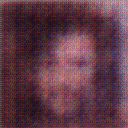
\includegraphics[width=150px]{500_fake_images/samples_5_224.png}%
\caption{A Black And White Cat Sitting On A Window Sill}%
\end{figure}

%
\end{document}